\documentclass[12pt, a4paper]{article}
\usepackage[utf8]{inputenc}
\usepackage[russian]{babel}
\usepackage[pdftex]{graphicx, color}
\usepackage{amsmath, amsfonts, amssymb, amsthm}
\usepackage[left=2cm,right=2cm,top=1.5cm,bottom=2cm]{geometry}
\usepackage{indentfirst}
\usepackage{hyperref}

\usepackage{setspace}
\onehalfspacing
\graphicspath{{pics/}}

\begin{document}
    \begin{singlespace}
    \begin{center}
        
\includegraphics[height=3cm]{msu.png}

        {\large\textbf{Отчёт по практическому заданию по БММО\\
        <<Байесовские рассуждения>>}\\
        Вариант 1}

        \vspace{0.3cm}

        \textit{\textbf{Аят Оспанов}}

        617 гр., ММП, ВМК МГУ, Москва

        20 сентября 2017 г.
    \end{center}
    \end{singlespace}

    \tableofcontents

    \section{Математические ожидания и дисперсии априорных распределений}
        \subsection{$p(a)$, $p(b)$}
            По условию $a \sim \text{Unif}[a_{min}, a_{max}]$, $b \sim \text{Unif}[b_{min}, b_{max}]$. Тогда матожидания и дисперсии считаются по определению:
            \begin{gather}
                \mathbb{E} a = \frac{a_{min} + a_{max}}{2} \\
                \mathbb{E} b = \frac{b_{min} + b_{max}}{2} \\
                \mathbb{D} a = \frac{(a_{max} - a_{min} + 1)^2 + 1}{12} \\
                \mathbb{D} b = \frac{(b_{max} - b_{min} + 1)^2 + 1}{12}
            \end{gather}

        \subsection{$p(c)$, $p(d)$}
            Воспользуемся следующими свойствами условных матожидания и дисперсии:
            $$\mathbb{E} X = \mathbb{E}\mathbb{E} [X | Y]$$
            $$\mathbb{D} X = \mathbb{E}\mathbb{D} [X | Y] + \mathbb{D}\mathbb{E} [X | Y]$$

            По условию, для модели 1, $c|a,b \sim \text{Bin}(a, p_1) + \text{Bin}(b, p_2)$; $d|c \sim c + \text{Bin}(c, p_3)$. Тогда:
            \begin{gather}
                \mathbb{E} c = \mathbb{E}_{a,b}\mathbb{E}_{c}[c|a,b] = \mathbb{E}_{a,b}[ap_1 + bp_2] = p_1 \mathbb{E} a + p_2 \mathbb{E} b \\
                \mathbb{E} d = \mathbb{E}_{c}\mathbb{E}_{d}[d|c] = \mathbb{E}_{c}[c + c p_3] = \mathbb{E}[c] + \mathbb{E}[c p_3] = (1 + p_3)\mathbb{E} c
            \end{gather}
            \begin{gather}
                \mathbb{D} c = \mathbb{E}_{a,b}\mathbb{D}_{c}[c|a,b] + \mathbb{D}_{a,b}\mathbb{E}_{c}[c|a,b] = \mathbb{E}_{a,b}[ap_1(1-p_1) + bp_2(1-p_2)] + \mathbb{D}_{a,b}[ap_1 + bp_2] = \nonumber\\
        = p_1 (1 - p_1) \mathbb{E} a + p_2 (1 - p_2) \mathbb{E} b + p_1^2 \mathbb{D} a + p_2^2 \mathbb{D} b\\
                \mathbb{D} d = \mathbb{E}_{c}\mathbb{D}_{d}[d|c] + \mathbb{D}_{c}\mathbb{E}_{d}[d|c] = \mathbb{E}_{c}[0 + c p_3(1 - p_3)] + \mathbb{D}_{c}[c + c p_3] = \nonumber\\ = p_3(1 - p_3) \mathbb{E}c + (1 + p_3)^2 \mathbb{D}c
            \end{gather}

            Для модели 2 $c|a,b \sim \text{Poiss}(ap_1 + bp_2)$. При этих условиях меняется только дисперсия:
            \begin{gather}
                \mathbb{D} c = \mathbb{E}_{a,b}\mathbb{D}_{c}[c|a,b] + \mathbb{D}_{a,b}\mathbb{E}_{c}[c|a,b] = \mathbb{E}_{a,b}[ap_1 + bp_2] + \mathbb{D}_{a,b}[ap_1 + bp_2] = \nonumber\\
        = p_1 \mathbb{E} a + p_2 \mathbb{E} b + p_1^2 \mathbb{D} a + p_2^2 \mathbb{D} b
            \end{gather}

        \subsection{Численные значения}
            \begin{center}
            \begin{tabular}{| l | c | c |}
                \hline
                & Модель 1 & Модель 2 \\
                \hline
                $\mathbb{E} a$ & 82.5 & 82.5 \\
                \hline
                $\mathbb{E} b$ & 550.0 & 550.0 \\
                \hline
                $\mathbb{E} c$ & 13.75 & 13.75 \\
                \hline
                $\mathbb{E} d$ & 17.875 & 17.875 \\
                \hline
                $\mathbb{D} a$ & 21.25 & 21.25 \\
                \hline
                $\mathbb{D} b$ & 850.0 & 850.0 \\
                \hline
                $\mathbb{D} c$ & 13.1675 & 14.0475 \\
                \hline
                $\mathbb{D} d$ & 25.1405 & 26.6277 \\
                \hline
            \end{tabular}
            \end{center}

    \section{Уточнение прогноза для величины $c$ по мере прихода новой косвенной информации}
        \subsection{Распределение $p(c)$}
            \begin{gather}
                p(c) = \sum_{a={a_{min}}}^{{a_{max}}} \sum_{b={b_{min}}}^{{b_{max}}} p(a, b, c) =
                \sum_{a={a_{min}}}^{{a_{max}}} \sum_{b={b_{min}}}^{{b_{max}}} p(c|a,b)p(a, b) =
                \sum_{a={a_{min}}}^{{a_{max}}} \sum_{b={b_{min}}}^{{b_{max}}} p(c|a,b)p(a)p(b) = \nonumber\\
                = p(a)p(b) \sum_{a={a_{min}}}^{{a_{max}}} \sum_{b={b_{min}}}^{{b_{max}}} p(c|a,b) =
                \{\text{формула свертки + смена порядка суммирования}\} = \nonumber\\
                = p(a)p(b)\sum_{k=0}^{a_{max} + b_{max}} \sum_{a={a_{min}}}^{{a_{max}}}p_A(k) \sum_{b={b_{min}}}^{{b_{max}}}p_B(a_{max} + b_{max}-k).
            \end{gather}
            Где:
            $$A \sim \text{Bin}(a,p_1), B \sim \text{Bin}(b,p_2) \text{ (для 1 модели)}$$
            $$A \sim \text{Poiss}(ap_1), B \sim \text{Poiss}(bp_2) \text{ (для 2 модели)}$$

        \subsection{Распределение $p(c|a)$}
            \begin{gather}
                p(c|a) = \sum_{b={b_{min}}}^{{b_{max}}} p(c|a,b) p(b) = p(b) \sum_{b={b_{min}}}^{{b_{max}}} p(c|a,b) = \nonumber\\
                \{\text{аналогично с } p(c)\}= p(b)\sum_{k=0}^{a_{max} + b_{max}} p_A(k) \sum_{b={b_{min}}}^{{b_{max}}}p_B(a_{max} + b_{max}-k).
            \end{gather}

        \subsection{Распределение $p(c|b)$}
            Аналогично с $p(c|a)$
            \begin{gather}
                p(c|b) = p(b)\sum_{k=0}^{a_{max} + b_{max}} p_B(a_{max} + b_{max}-k) \sum_{a={a_{min}}}^{{a_{max}}}p_A(k).
            \end{gather}

        \subsection{Распределение $p(c|d)$}
            \begin{gather}
                p(c|d) = \frac{p(d|c)p(c)}{p(d)} \propto p(d|c)p(c)
            \end{gather}

        \subsection{Распределение $p(c|a,b,d)$}
            \begin{gather}
                p(c|a,b,d) = \frac{p(a,b,c,d)}{p(a,b,d)} = \frac{p(d|c)p(c|a,b)p(a)p(b)}{p(a,b,d)} \propto p(d|c)p(c|a,b)
            \end{gather}

        \subsection{Наблюдение}
            \begin{figure}
                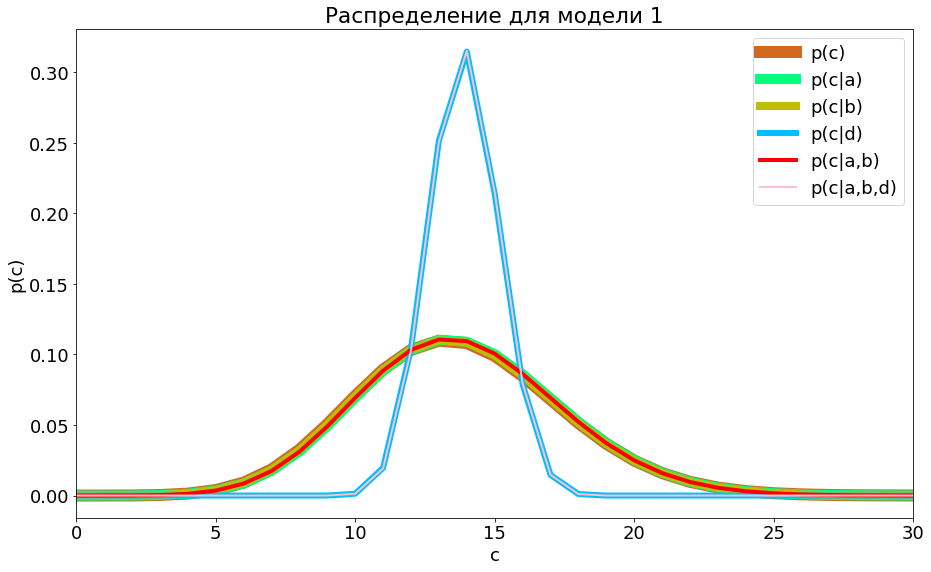
\includegraphics[width=\linewidth]{model1}
                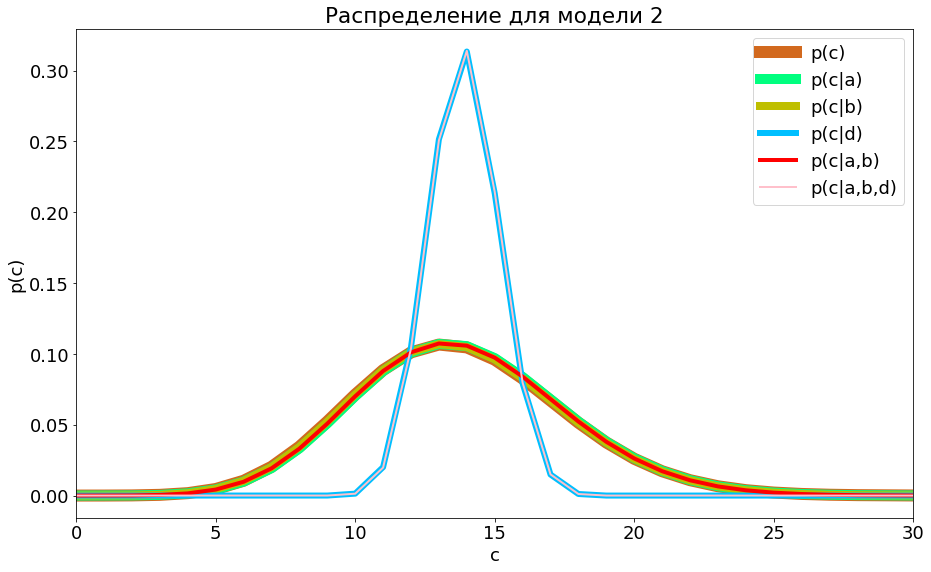
\includegraphics[width=\linewidth]{model2}
                \caption{Распределения вероятностей}
                \label{fig:m1}
            \end{figure}

            Из Рис. \ref{fig:m1} видно, что добавление информации о количестве студентов ($a$, $b$) не уточняет прогноз для величины $c$. Но добавление информации о записавшихся на лекцию ($d$) существенно уточняет прогноз. Также видна похожесть графиков $p(c|d)$ и $p(c|a,b,d)$, что подтверждает, что $a$ и $b$ не влияют на прогноз.

            Из Таблиц \ref{tab:m1} и \ref{tab:m2} можно понять насколько идет уточнение. В случае добавления $a$ и $b$ дисперсия уменьшается по сравнению с $p(c)$, но меняется незначительно. А при добавлении $d$ дисперсия значительно снижается, что показывает хорошое уточнение прогноза.

            \begin{table}[h]
                \caption{Модель 1}
                \label{tab:m1}
                \begin{tabular}{l | l | l | l | l | l | l}
                & \textbf{p(c)} & \textbf{p(c|a)} & \textbf{p(c|b)} & \textbf{p(c|d)} & \textbf{p(c|a,b)} & \textbf{p(c|a,b,d)} \\
                \hline
                Матожидание & 13.7500 & 13.8 & 13.7500 & 13.895971 & 13.800 & 13.902756 \\
                Дисперсия & 13.1675 & 13.0 & 13.0825 & 1.533582 & 12.915 & 1.530140 \\
                \end{tabular}
            \end{table}

            \begin{table}[h]
                \caption{Модель 2}
                \label{tab:m2}
                \begin{tabular}{l | l | l | l | l | l | l}
                & \textbf{p(c)} & \textbf{p(c|a)} & \textbf{p(c|b)} & \textbf{p(c|d)} & \textbf{p(c|a,b)} & \textbf{p(c|a,b,d)} \\
                \hline
                Матожидание & 13.7500 & 13.8 & 13.7500 & 13.893834 & 13.8 & 13.900175 \\
                Дисперсия & 14.0475 & 13.885 & 13.9625 & 1.543943 & 13.8 & 1.540884 \\
                \end{tabular}
            \end{table}

            Также по таблицам видно, что 2 модель показывает примерно те же матожидания, что и 1 модель, но дисперсии чуть больше, т.к. 2 модель является приближением 1 модели, что приводит к потере точности.

    \section{Наибольший вклад в уточнение прогноза для величины $c$}
        Программным путем было выяснено, что для допустимых значений $a, b, d$ верны выражения $\mathbb{D}[c|d] < \mathbb{D}[c|a], \mathbb{D}[c|d] < \mathbb{D}[c|b]$:
            \begin{center}
            \begin{tabular}{l | l | l | l}
                \textbf{Модель} & $\max{\mathbb{D}[c|d]}$ & $\min{\mathbb{D}[c|a]}$ & $\min{\mathbb{D}[c|b]}$\\
                \hline
                1 & 10.2986909051 & 12.28 & 12.5875\\
                2 & 12.8941557054 & 13.085 & 13.4625\\
            \end{tabular}
            \end{center}

        Далее вычислим множество точек $(a, b)$ таких, что $\mathbb{D}[c|b] < \mathbb{D}[c|a]$:
        \begin{gather}
            \mathbb{D}_c[c|a] = \mathbb{E}_b\mathbb{D}_c[c|a,b] + \mathbb{D}_b\mathbb{E}_c[c|a,b] =
            \mathbb{E}_b[ap_1(1-p_1) + bp_2(1-p_2)] + \mathbb{D}_b[ap_1 + bp_2] = \nonumber \\
            = ap_1(1-p_1) + p_2(1-p_2)\mathbb{E}b + p_2^2\mathbb{D}b.
        \end{gather}

        Аналогично:
        \begin{gather}
            \mathbb{D}_c[c|b] = p_1(1-p_1)\mathbb{E}a + bp_2(1-p_2) + p_1^2\mathbb{D}a.
        \end{gather}

        Далее решим $\mathbb{D}[c|b] < \mathbb{D}[c|a]$:
        \begin{gather}
            p_1(1-p_1)\mathbb{E}a + bp_2(1-p_2) + p_1^2\mathbb{D}a < ap_1(1-p_1) + p_2(1-p_2)\mathbb{E}b + p_2^2\mathbb{D}b \nonumber \\
            bp_2(1-p_2) - ap_1(1-p_1) < p_2(1-p_2)\mathbb{E}b + p_2^2\mathbb{D}b - p_1(1-p_1)\mathbb{E}a - p_1^2\mathbb{D}a \nonumber
        \end{gather}
        $$
        \text{Пусть } A = p_1(1 - p_1); B = p_2(1 - p_2);
        $$
        $$
        C = p_2(1-p_2)\mathbb{E}b + p_2^2\mathbb{D}b - p_1(1-p_1)\mathbb{E}a - p_1^2\mathbb{D}a
        $$
        Тогда видно, что неравенство линейное относительно $(a,b)$:
        \begin{gather}
            Bb - Aa < C
        \end{gather}
        Следовательно для $\mathbb{D}[c|b] \geq \mathbb{D}[c|a]$: $Bb - Aa \geq C$. Это и означает линейную разделимость множеств $\{(a, b) | \mathbb{D}[c|b] < \mathbb{D}[c|a] \}$ и $\{(a, b) | \mathbb{D}[c|b] \geq \mathbb{D}[c|a]\}$ прямой $Bb - Aa = C$.

        Для модели 2 линейность сохраняется и меняются лишь константы.

    \section{Временные замеры}\label{sec:time}
        \begin{table}[h]
            \caption{Время вычислений распределений, в сек}
            \label{tab:time}
            \begin{tabular}{l | l | l | l | l | l | l | l}
            \textbf{Модель} & \textbf{p(c)} & \textbf{p(c|a)} & \textbf{p(c|b)} & \textbf{p(c|d)} & \textbf{p(c|a,b)} & \textbf{p(c|a,b,d)} & \textbf{p(d)}\\
            \hline
            1 & 0.012417 & 0.011621 & 0.000789 & 0.011432 & 0.000493 & 0.000585 & 0.072148\\
            2 & 0.005038 & 0.004840 & 0.000393 & 0.005094 & 0.000146 & 0.000253 & 0.068229\\
            \end{tabular}
        \end{table}

    \section{Сравнение результатов для двух моделей}
        При апроксимации биномиального распределения пуассоновским распределением, мы отметили, что можем с высокой точностью приблизить при большом количестве испытаний и маленькой вероятности успеха. Следовательно, максимальная разница проявляется при высоких вероятностях успеха. Например, возьмем $p_1 = p_2 = 0.99$ ($a = 100, b = 200$). Тогда:
        \begin{gather}
        \mathbb{D}c = 2.0746983826247742 \text{ для модели 1}\nonumber\\
        \mathbb{D}c = 296.99999999816646 \text{ для модели 1}\nonumber
        \end{gather}

        Но, как показывает таблица из пункта \ref{sec:time}, такая аппроксимация дает прирост в среднем на 2 раза. Если выполнены условия аппроксимации и важно время выполнения, то можно использовать модель 2, но в целом лучше использовать модель 1.


\end{document}
